% !TeX spellcheck = en_GB
\documentclass[
	9pt,
	a4paper,
	handout
]{beamer}
\usetheme{Frankfurt}
\usepackage{lmodern}
\beamertemplatenavigationsymbolsempty


%\setbeamercolor{section in head/foot}{fg=white, bg=gray!70!black}
\definecolor{navbar}{rgb}{0.10, 0.10, 0.45}
\setbeamercolor{section in head/foot}{fg=white, bg=navbar}
\setbeamertemplate{footline}
{
	\definecolor{headerblue}{rgb}{0.2, 0.2, 0.7}
	\setbeamercolor{footblue}{fg=white, bg=headerblue}
	\definecolor{defblue}{rgb}{0.15, 0.15, 0.55}
	\setbeamercolor{darkfootblue}{fg=white, bg=defblue}
	\leavevmode%
	\hbox{%
		\begin{beamercolorbox}[wd=.25\paperwidth, ht=2.25ex, dp=1ex, center]{darkfootblue}%
			\usebeamerfont{author in head/foot}Zeno Adrian Weil
		\end{beamercolorbox}%
		\begin{beamercolorbox}[wd=.5\paperwidth, ht=2.25ex, dp=1ex, center]{footblue}%
			\usebeamerfont{title in head/foot} Stream Mining: One-Hot Encoding and DGIM
		\end{beamercolorbox}%
		\begin{beamercolorbox}[wd=.25\paperwidth, ht=2.25ex, dp=1ex, right]{darkfootblue}%
			\usebeamerfont{date in head/foot}\insertshortdate{}\hspace*{2em}
			\insertframenumber{} / \inserttotalframenumber\hspace*{2ex} 
	\end{beamercolorbox}}%
	\vskip0pt%
}


\usepackage[english]{babel}
\usepackage{hyperref}
\usepackage{amsmath}
\usepackage{pifont}
\newcommand{\cmark}{\ding{51}}%
\newcommand{\xmark}{\ding{55}}%
\usepackage{tikz}

%%% dicke, verschiedenfarbige Hervorhebungen
\newcommand{\emphblue}[1]{{\color{blue!80!black}\textbf{#1}}}
\newcommand{\emphred}[1]{{\color{red!85!black}\textbf{#1}}}
\newcommand{\emphblack}[1]{\textbf{#1}}
\newcommand{\emphmathblack}[1]{{\color{black}$\boldsymbol{#1}$}}
\newcommand{\emphmathblue}[1]{{\color{blue!80!black}$\boldsymbol{#1}$}}
\newcommand{\mathemphmm}[1]{{\color{blue!80!black}\textbf{$#1$}}}


%%% Zeichen aus pifont
\newcommand{\cmark}{\ding{51}}  % ✔
\newcommand{\xmark}{\ding{55}}  % ✘

\title{Stream Mining}
\subtitle{One-Hot Encoding and DGIM}
\author{Zeno Adrian Weil}
\institute{Data Science 1 \\ Goethe University Frankfurt}
\date{7th June 2022}

\begin{document}
	\begin{frame}[plain]
		\titlepage
	\end{frame}

	\section{One-Hot Encoding}
	% !TeX spellcheck = en_GB
\begin{frame}[t]{One-Hot Encoding}
	\begin{itemize}
		\item
		categorical features
		\begin{itemize}
			\item
			nominal (e.g. colours)
			
			\item
			ordinal (e.g. satisfaction levels)
		\end{itemize}
	
		\item
		need for numbers in algorithms
	
		\item
		naive approach: number serially
		\begin{itemize}
			\item
			may introduce arbitrary orders
			
			\item
			calculating non-sensical differences
		\end{itemize}
	
		\item
		one-hot encoding
		\begin{itemize}
			\item
			one binary feature for each possible value
		\end{itemize}
	\end{itemize}
\end{frame}

	\section{The DGIM Algorithm}
	% !TeX spellcheck = en_GB
\begin{frame}{The Datar-Gionis-Indyk-Motwani Algorithm}
	\begin{block}{Objectives}<2->
		\begin{itemize}
			\item<3->
			\emphblack{Estimate} the number of \emphblack{ones} in a bit stream!

			\item<4->
			Be \emphblack{space-efficient}!
		\end{itemize}
	\end{block}
	\begin{itemize}
		\item<5->
		window size $N$

		\item<6->
		$\mathcal{O}(\log_2 N)$ \emphblue{buckets}
		\begin{itemize}
			\item<8->
			\emphblack{timestamp}

			\item<9->
			\emphblack{size} = number of ones
			\begin{itemize}
				\item<10->
				powers of two
%
%				\item
%				one or two of each size
			\end{itemize}

			\item<11->
			include all ones; end with ones
		\end{itemize}
	
		\item<12->
		\emphblue{estimation}: half the size of the oldest bucket + sum of sizes of all other buckets
		\begin{itemize}
			\item<15->
			error rate: $\pm50\%$
		\end{itemize}
	
		\item<16->
		needs only \emphmathblack{\mathcal{O}( \!\!\:(\log_2 N)^2 )} \emphblack{bits}
	\end{itemize}
	%
	\begin{center}
		\begin{tikzpicture}[node distance=1mm]
			% bits
			\onslide<7->{
				\tikzstyle{every node} = [font={\large}]
				\node[draw] (a) {$\dots 1 ~ 0 ~ 1$};
				\node[draw, right=of a] (b) {$1 ~ 0 ~ 1 ~ 1 ~ 0 ~ 0 ~ 0 ~ 1$};
				\node[right=of b] (c) {$0$};
				\node[draw, right=of c] (d) {$1 ~ 1 ~ 1 ~ 0 ~ 1$};
				\node[draw, right=of d] (e) {$1 ~ 0 ~ 0 ~ 1$};
				\node[right=of e] (f) {$0$};
				\node[draw, right=of f] (g) {$1$};
				\node[draw, right=of g] (h) {$1$};
				\node[right=of h] (i) {$0$};
			}
			% bucket sizes
			\onslide<9->{
				\tikzstyle{every node} = [font={\small}]
				\node[above=0mm of a] {sizes: 8};
				\node[above=0mm of b] {4};
				\node[above=0mm of d] {4};
				\node[above=0mm of e] {2};
				\node[above=0mm of g] {1};
				\node[above=0mm of h] {1};
			}
		\end{tikzpicture}
	\end{center}
	%
	\begin{center}
		\small
		\onslide<13->{estimation:~16}
		\qquad\qquad
		\onslide<14->{reality:~14}
	\end{center}
\end{frame}
	
	\section{The Mushroom Data Set}
	% !TeX spellcheck = en_GB
\begin{frame}{The Mushroom Data Set (J.S. Schlimmer, 1987)}
	\begin{itemize}
		\item
		\emphblue{8124 samples} of 23 mushroom species
		\begin{itemize}
			\item
			4208 edible
			
			\item
			3916 poisonous
		\end{itemize}
	
		\item
		\emphblue{22 attributes} with 128 possible values
		
		\item
		saved as CSV
	\end{itemize}

	\begin{center}
		\texttt{p,x,s,n,t,p,f,c,n,k,e,e,s,s,w,w,p,w,o,p,k,s,u}

		\texttt{e,x,s,y,t,a,f,c,b,k,e,c,s,s,w,w,p,w,o,p,n,n,g}

		\texttt{e,b,s,w,t,l,f,c,b,n,e,c,s,s,w,w,p,w,o,p,n,n,m}

		\dots
	\end{center}

	\medspace

	\begin{block}{}
		Are there simple rules to determine edibility?
		\emphblack{Yes!}
	\end{block}
\end{frame}
	
	\section{The Implementation}
	% !TeX spellcheck = en_GB
\begin{frame}{The Implementation}
	\begin{itemize}
		\item
		load CSV with Python

		\item
		\emphblack{2D array} for the one-hot encoding of the odour
		
		\item
		Python package \emphblack{dgim} for the algorithm
		
		\item
		\emphblack{Streamlit} for the interface
		
		\item
		options
		\begin{itemize}
			\item
			odour type
			
			\item
			window size $N$
			
			\item
			error rate
		\end{itemize}
	\end{itemize}

	\begin{picture}(0,0)(-215,-5)
		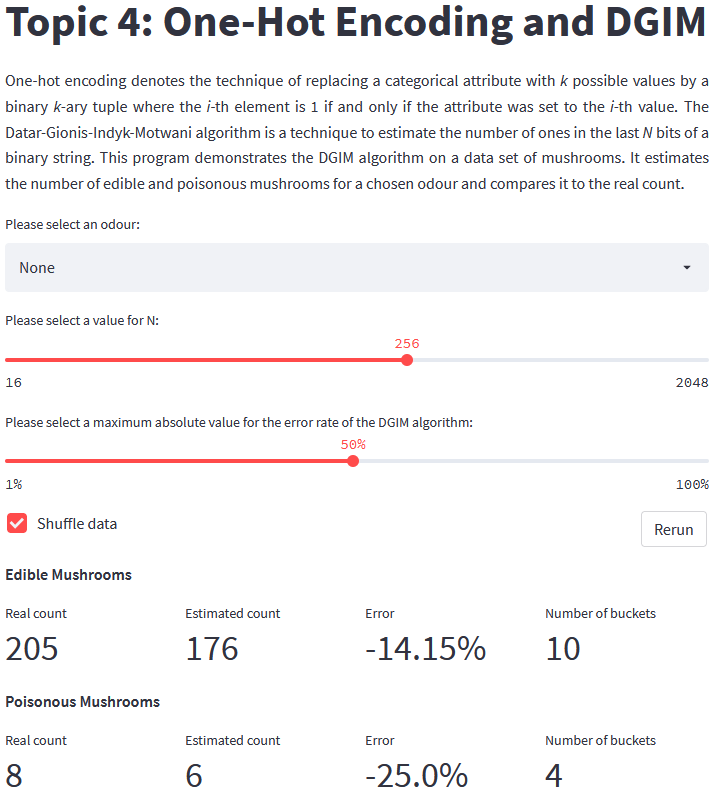
\includegraphics[height=4cm]{images/overview.png}
	\end{picture}
\end{frame}

\begin{frame}[plain]{}
	\begin{figure}
		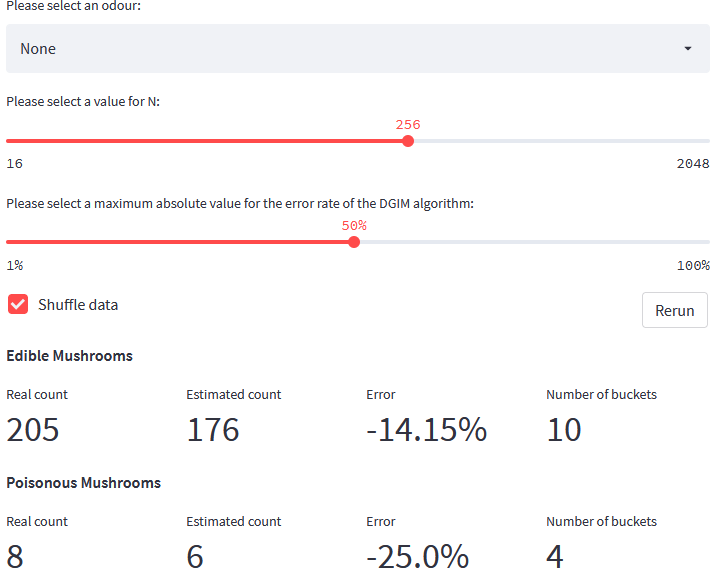
\includegraphics[height=.75\linewidth]{images/typical1.png}
	\end{figure}
\end{frame}

\begin{frame}[plain]{}
	\begin{figure}
		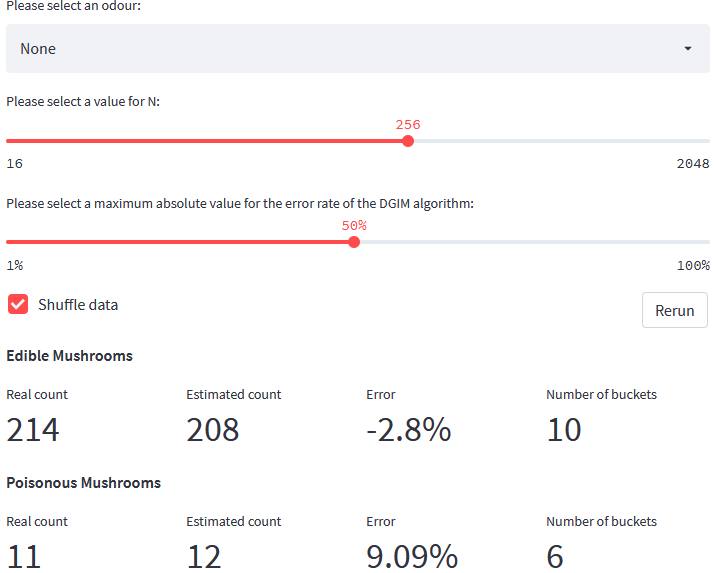
\includegraphics[height=.75\linewidth]{images/typical2.png}
	\end{figure}
\end{frame}

\begin{frame}[plain]{}
	\begin{figure}
		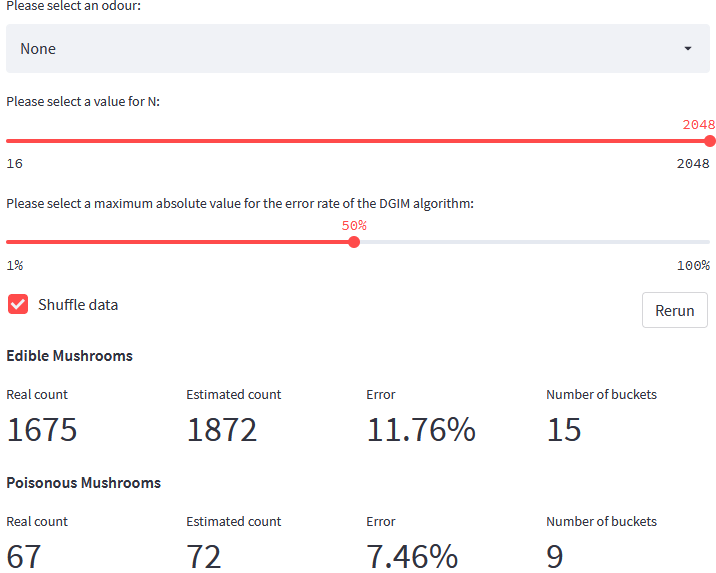
\includegraphics[height=.75\linewidth]{images/big_n.png}
	\end{figure}
\end{frame}

\begin{frame}[plain]{}
	\begin{figure}
		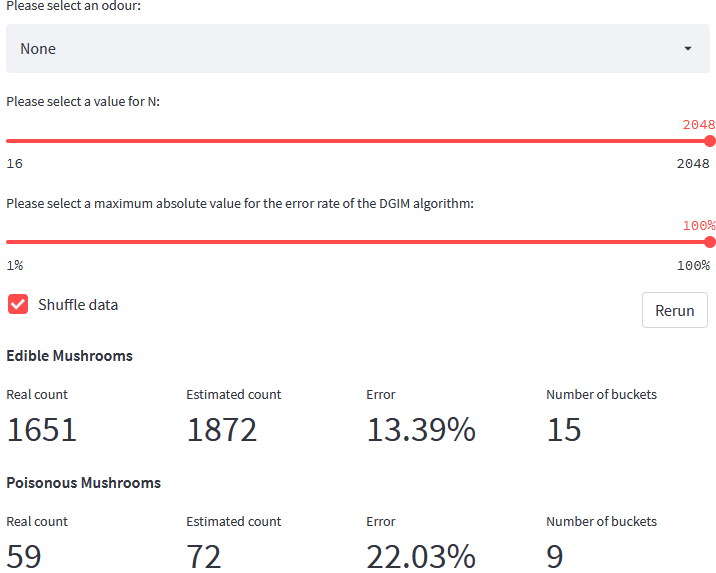
\includegraphics[height=.75\linewidth]{images/big_e.png}
	\end{figure}
\end{frame}

\begin{frame}[plain]{}
	\begin{figure}
		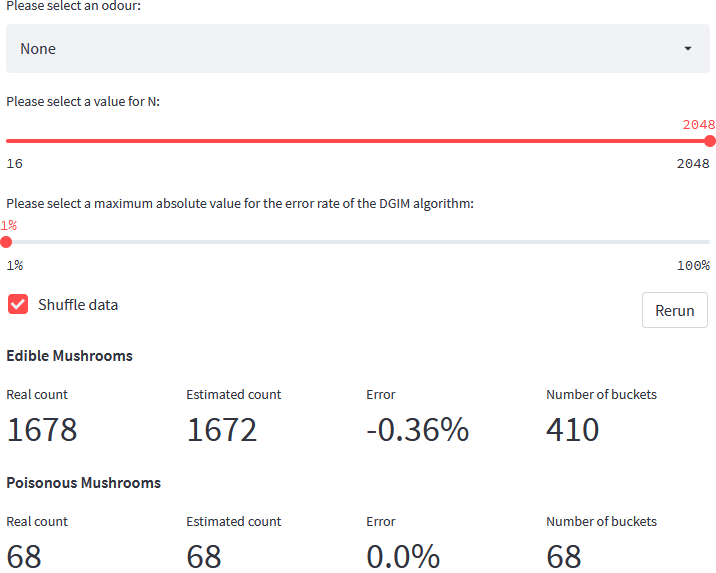
\includegraphics[height=.75\linewidth]{images/small_e.png}
	\end{figure}
\end{frame}

	\section{References}
	% !TeX spellcheck = en_GB
\begin{frame}{References}
	\begin{itemize}
		\item
		Project code:
		\url{https://github.com/s9770652/DS1-DGIM}
		
		\item
		Mushroom data set:
		\url{https://archive-beta.ics.uci.edu/ml/datasets/mushroom}
		
		\item
		Streamlit:
		\url{https://streamlit.io/}
		
		\item
		Python package \emph{dgim}:
		\url{https://pypi.org/project/dgim/}
		
		\item
		Description of one-hot encoding:
		\url{https://sherbold.github.io/intro-to-data-science/04_Data-Analysis-Overview.html\#Features}
		
		\item
		Description of the DGIM algorithm:
		\url{http://infolab.stanford.edu/~ullman/mmds/ch4.pdf}
	\end{itemize}
\end{frame}
\end{document}